% ****************************************************************************************
% ********************    FUNCIONES, CALCULO DIFERENCIAL, INTEGRAL     *******************
% ****************************************************************************************


% =======================================================
% =======         HEADER FOR DOCUMENT        ============
% =======================================================
    
    % *********  SPECIFIC FOR THIS BOOK  ********
    \def\ProjectAuthorLink{https://github.com/CompilandoConocimiento}
    \def\ProjectNameLink{\ProjectAuthorLink/LibroCalculoDiferencialEIntegral}    
    

    % *********   DOCUMENT ITSELF   **************
    \documentclass[12pt, fleqn]{report}                             %Type of doc and size of font and left equations
    \usepackage[margin=1.2in]{geometry}                             %Margins and Geometry pacakge
    \usepackage{ifthen}                                             %Allow simple programming using if - then
    \usepackage[hidelinks]{hyperref}                                %Allow to create hiperlinks and Fuck Firefox
    \usepackage{pdfpages}                                           %Allow us 'import' PDF's
    \hypersetup{pageanchor=false}                                   %Solve 'double page 1' warnings in build :v
    \setlength{\parindent}{0pt}                                     %Eliminate ugly indentation
    \author{Oscar Andrés Rosas}                                     %Who I am

    % *********   LANGUAJE    *****************
    \usepackage[spanish]{babel}                                     %Please allow me to type in spanish
    \usepackage[utf8]{inputenc}                                     %Lets use UFT-8
    \usepackage[T1]{fontenc}                                        %Allow for better font support
    \usepackage{textcmds}                                           %Allow us to use quoutes
    \usepackage{changepage}                                         %Allow us to use identate paragraphs
    \usepackage{anyfontsize}                                        %All the sizes for fonts wiiiii!

    % *********   MATH AND HIS STYLE  *********
    \usepackage{ntheorem, amsmath, amssymb, amsfonts}               %All fucking math, I want all!
    \usepackage{mathrsfs, mathtools, empheq}                        %All fucking math, I want all!
    \usepackage{cancel}                                             %Negate symbol
    \usepackage{centernot}                                          %Allow me to negate a symbol
    \decimalpoint                                                   %Use decimal point

    % *********   GRAPHICS AND IMAGES *********
    \usepackage{graphicx}                                           %Allow to create graphics
    \usepackage{float}                                              %For images
    \usepackage{wrapfig}                                            %Allow to create images
    \graphicspath{ {Graphics/} }                                    %Where are the images :D

    % *********   LISTS AND TABLES ***********
    \usepackage{listings, listingsutf8}                             %We will be using code here
    \usepackage[inline]{enumitem}                                   %We will need to enumarate
    \usepackage{tasks}                                              %Horizontal lists
    \usepackage{longtable}                                          %Lets make tables awesome
    \usepackage{booktabs}                                           %Lets make tables awesome
    \usepackage{tabularx}                                           %Lets make tables awesome
    \usepackage{multirow}                                           %Lets make tables awesome
    \usepackage{multicol}                                           %Create multicolumns

    % *********   REMOVE SOME ERRORS **********
    \hbadness=10000                                                 %Ignore \vbox and \hbox warings
    \hfuzz=\maxdimen\newdimen\hfuzz                                 %Ignore \vbox and \hbox warings

    % *********   HEADERS AND FOOTERS ********
    \usepackage{fancyhdr}                                           %Lets make awesome headers/footers
    \pagestyle{fancy}                                               %Lets make awesome headers/footers
    \setlength{\headheight}{16pt}                                   %Top line
    \setlength{\parskip}{0.5em}                                     %Top line
    \renewcommand{\footrulewidth}{0.5pt}                            %Bottom line

    \lhead {                                                        %Left Header
        \hyperlink{chapter.\arabic{chapter}}                        %Make a link to the current chapter
        {\normalsize{\textsc{\nouppercase{\leftmark}}}}             %And fot it put the name
    }

    \rhead {                                                        %Right Header
        \hyperlink{section.\arabic{chapter}.\arabic{section}}       %Make a link to the current chapter
            {\footnotesize{\textsc{\nouppercase{\rightmark}}}}      %And fot it put the name
    }

    \rfoot{\textsc{\small{\hyperref[sec:Index]{Ve al Índice}}}}     %This will always be a footer  

    \fancyfoot[L]{                                                  %Algoritm for a changing footer
        \ifthenelse{\isodd{\value{page}}}                           %IF ODD PAGE:
            {\href{https://SoyOscarRH.github.io/}                   %DO THIS:
                {\footnotesize                                      %Send the page
                    {\textsc{Oscar Andrés Rosas}}}}                 %Send the page
            {\href{https://compilandoconocimiento.com}              %ELSE DO THIS: 
                {\footnotesize                                      %Send the author
                    {\textsc{Compilando Conocimiento}}}}            %Send the author
    }
    
    
% =======================================================
% ===================   COMMANDS    =====================
% =======================================================

    % =========================================
    % =======   NEW ENVIRONMENTS   ============
    % =========================================
    \newenvironment{Indentation}[1][0.75em]                         %Use: \begin{Inde...}[Num]...\end{Inde...}
        {\begin{adjustwidth}{#1}{}}                                 %If you dont put nothing i will use 0.75 em
        {\end{adjustwidth}}                                         %This indentate a paragraph
    
    \newenvironment{SmallIndentation}[1][0.75em]                    %Use: The same that we upper one, just 
        {\begin{adjustwidth}{#1}{}\begin{footnotesize}}             %footnotesize size of letter by default
        {\end{footnotesize}\end{adjustwidth}}                       %that's it
    
    \def \Eq {equation}                                             %Stupid Visual studio error
    \newenvironment{MultiLineEquation}[1]                           %Use: To create MultiLine equations
        {\begin{\Eq}\begin{alignedat}{#1}}                          %Use: \begin{Multi..}{Num. de Columnas}
        {\end{alignedat}\end{\Eq}}                                  %And.. that's it!
    
    \newenvironment{MultiLineEquation*}[1]                          %Use: To create MultiLine equations
        {\begin{\Eq*}\begin{alignedat}{#1}}                         %Use: \begin{Multi..}{Num. de Columnas}
        {\end{alignedat}\end{\Eq*}}                                 %And.. that's it!
    

    % =========================================
    % == GENERAL TEXT & SYMBOLS ENVIRONMENTS ==
    % =========================================
    
    % =====  TEXT  ======================
    \newcommand \Quote              {\qq}                           %Use: \Quote to use quotes
    \newcommand \Over               {\overline}                     %Use: \Bar to use just for short
    \newcommand \ForceNewLine       {$\Space$\\}                    %Use it in theorems for example
    \newcommand \ForceColumnBreak   {\vfill\null\columnbreak}       %Use only in multicols

    % =====  SPACES  ====================
    \DeclareMathOperator \Space     {\quad}                         %Use: \Space for a cool mega space
    \DeclareMathOperator \MegaSpace {\quad \quad}                   %Use: \MegaSpace for a cool mega mega space
    \DeclareMathOperator \MiniSpace {\;}                            %Use: \Space for a cool mini space
    
    % =====  MATH TEXT  =================
    \newcommand \Such           {\MiniSpace | \MiniSpace}           %Use: \Such like in sets
    \newcommand \Also           {\MiniSpace \text{y} \MiniSpace}    %Use: \Also so it's look cool
    \newcommand \Remember[1]    {\Space\text{\scriptsize{#1}}}      %Use: \Remember so it's look cool
    
    % =====  THEOREMS: IN SPANISH :0  ===
    \newtheorem{Theorem}        {Teorema}[section]                  %Use: \begin{Theorem}[Name]\label{Nombre}...
    \newtheorem{Corollary}      {Colorario}[Theorem]                %Use: \begin{Corollary}[Name]\label{Nombre}...
    \newtheorem{Lemma}[Theorem] {Lemma}                             %Use: \begin{Lemma}[Name]\label{Nombre}...
    \newtheorem{Definition}     {Definición}[section]               %Use: \begin{Definition}[Name]\label{Nombre}...
    \theoremstyle{break}                                            %THEOREMS START 1 SPACE AFTER Fuck!

    % =====  LOGIC  =====================
    \newcommand \lIff    {\leftrightarrow}                          %Use: \lIff for logic iff
    \newcommand \lEqual  {\MiniSpace \Leftrightarrow \MiniSpace}    %Use: \lEqual for a logic double arrow
    \newcommand \lInfire {\MiniSpace \Rightarrow \MiniSpace}        %Use: \lInfire for a logic infire
    \newcommand \lLongTo {\longrightarrow}                          %Use: \lLongTo for a long arrow

    % =====  FAMOUS SETS  ===============
    \DeclareMathOperator \Naturals     {\mathbb{N}}                 %Use: \Naturals por Notation
    \DeclareMathOperator \Primes       {\mathbb{P}}                 %Use: \Primes por Notation
    \DeclareMathOperator \Integers     {\mathbb{Z}}                 %Use: \Integers por Notation
    \DeclareMathOperator \Racionals    {\mathbb{Q}}                 %Use: \Racionals por Notation
    \DeclareMathOperator \Reals        {\mathbb{R}}                 %Use: \Reals por Notation
    \DeclareMathOperator \Complexs     {\mathbb{C}}                 %Use: \Complex por Notation
    \DeclareMathOperator \GenericField {\mathbb{F}}                 %Use: \GenericField por Notation
    \DeclareMathOperator \VectorSet    {\mathbb{V}}                 %Use: \VectorSet por Notation
    \DeclareMathOperator \SubVectorSet {\mathbb{W}}                 %Use: \SubVectorSet por Notation
    \DeclareMathOperator \Polynomials  {\mathbb{P}}                 %Use: \Polynomials por Notation
    \DeclareMathOperator \VectorSpace  {\VectorSet_{\GenericField}} %Use: \VectorSpace por Notation
    \DeclareMathOperator \LinealTransformation {\mathcal{T}}        %Use: \LinealTransformation for a cool T
    \DeclareMathOperator \LinTrans      {\mathcal{T}}               %Use: \LinTrans for a cool T
    \DeclareMathOperator \Laplace       {\mathcal{L}}               %Use: \LinTrans for a cool T

    % =====  CONTAINERS   ===============
    \newcommand{\Set}[1]            {\left\{ \; #1 \; \right\}}     %Use: \Set {Info} for INTELLIGENT space 
    \newcommand{\bigSet}[1]         {\big\{  \; #1 \; \big\}}       %Use: \bigSet  {Info} for space 
    \newcommand{\BigSet}[1]         {\Big\{  \; #1 \; \Big\}}       %Use: \BigSet  {Info} for space 
    \newcommand{\biggSet}[1]        {\bigg\{ \; #1 \; \bigg\}}      %Use: \biggSet {Info} for space 
    \newcommand{\BiggSet}[1]        {\Bigg\{ \; #1 \; \Bigg\}}      %Use: \BiggSet {Info} for space 
        
    \newcommand{\Wrap}[1]           {\left( #1 \right)}             %Use: \Wrap {Info} for INTELLIGENT space
    \newcommand{\bigWrap}[1]        {\big( \; #1 \; \big)}          %Use: \bigBrackets  {Info} for space 
    \newcommand{\BigWrap}[1]        {\Big( \; #1 \; \Big)}          %Use: \BigBrackets  {Info} for space 
    \newcommand{\biggWrap}[1]       {\bigg( \; #1 \; \bigg)}        %Use: \biggBrackets {Info} for space 
    \newcommand{\BiggWrap}[1]       {\Bigg( \; #1 \; \Bigg)}        %Use: \BiggBrackets {Info} for space 

    \newcommand{\Brackets}[1]       {\left[ #1 \right]}             %Use: \Brackets {Info} for INTELLIGENT space
    \newcommand{\bigBrackets}[1]    {\big[ \; #1 \; \big]}          %Use: \bigBrackets  {Info} for space 
    \newcommand{\BigBrackets}[1]    {\Big[ \; #1 \; \Big]}          %Use: \BigBrackets  {Info} for space 
    \newcommand{\biggBrackets}[1]   {\bigg[ \; #1 \; \bigg]}        %Use: \biggBrackets {Info} for space 
    \newcommand{\BiggBrackets}[1]   {\Bigg[ \; #1 \; \Bigg]}        %Use: \BiggBrackets {Info} for space 

    \newcommand{\Generate}[1]   {\left\langle #1 \right\rangle}     %Use: \Generate {Info} <>
    \newcommand{\Floor}[1]      {\left \lfloor #1 \right \rfloor}   %Use: \Floor {Info} for floor 
    \newcommand{\Ceil}[1]       {\left \lceil #1 \right \rceil }    %Use: \Ceil {Info} for ceil
    
    % =====  BETTERS MATH COMMANDS   =====
    \newcommand{\pfrac}[2]      {\Wrap{\dfrac{#1}{#2}}}             %Use: Put fractions in parentesis

    % =========================================
    % ====   LINEAL ALGEBRA & VECTORS    ======
    % =========================================

    % ===== UNIT VECTORS  ================
    \newcommand{\hati}      {\hat{\imath}}                           %Use: \hati for unit vector    
    \newcommand{\hatj}      {\hat{\jmath}}                           %Use: \hatj for unit vector    
    \newcommand{\hatk}      {\hat{k}}                                %Use: \hatk for unit vector

    % ===== MAGNITUDE  ===================
    \newcommand{\abs}[1]    {\left\lvert #1 \right\lvert}           %Use: \abs{expression} for |x|
    \newcommand{\Abs}[1]    {\left\lVert #1 \right\lVert}           %Use: \Abs{expression} for ||x||
    \newcommand{\Mag}[1]    {\left| #1 \right|}                     %Use: \Mag {Info} 
    
    \newcommand{\bVec}[1]   {\mathbf{#1}}                           %Use for bold type of vector
    \newcommand{\lVec}[1]   {\overrightarrow{#1}}                   %Use for a long arrow over a vector
    \newcommand{\uVec}[1]   {\mathbf{\hat{#1}}}                     %Use: Unitary Vector Example: $\uVec{i}

    % ===== FN LINEAL TRANSFORMATION  ====
    \newcommand{\FnLinTrans}[1]{\mathcal{T}\Wrap{#1}}               %Use: \FnLinTrans for a cool T
    \newcommand{\VecLinTrans}[1]{\mathcal{T}\pVector{#1}}           %Use: \LinTrans for a cool T
    \newcommand{\FnLinealTransformation}[1]{\mathcal{T}\Wrap{#1}}   %Use: \FnLinealTransformation

    % ===== ALL FOR DOT PRODUCT  =========
    \makeatletter                                                   %WTF! IS THIS
    \newcommand*\dotP{\mathpalette\dotP@{.5}}                       %Use: \dotP for dot product
    \newcommand*\dotP@[2] {\mathbin {                               %WTF! IS THIS            
        \vcenter{\hbox{\scalebox{#2}{$\m@th#1\bullet$}}}}           %WTF! IS THIS
    }                                                               %WTF! IS THIS
    \makeatother                                                    %WTF! IS THIS

    % === WRAPPERS FOR COLUMN VECTOR ===
    \newcommand{\pVector}[1]                                        %Use: \pVector {Matrix Notation} use parentesis
        { \ensuremath{\begin{pmatrix}#1\end{pmatrix}} }             %Example: \pVector{a\\b\\c} or \pVector{a&b&c} 
    \newcommand{\lVector}[1]                                        %Use: \lVector {Matrix Notation} use a abs 
        { \ensuremath{\begin{vmatrix}#1\end{vmatrix}} }             %Example: \lVector{a\\b\\c} or \lVector{a&b&c} 
    \newcommand{\bVector}[1]                                        %Use: \bVector {Matrix Notation} use a brackets 
        { \ensuremath{\begin{bmatrix}#1\end{bmatrix}} }             %Example: \bVector{a\\b\\c} or \bVector{a&b&c} 
    \newcommand{\Vector}[1]                                         %Use: \Vector {Matrix Notation} no parentesis
        { \ensuremath{\begin{matrix}#1\end{matrix}} }               %Example: \Vector{a\\b\\c} or \Vector{a&b&c}

    % === MAKE MATRIX BETTER  =========
    \makeatletter                                                   %Example: \begin{matrix}[cc|c]
    \renewcommand*\env@matrix[1][*\c@MaxMatrixCols c] {             %WTF! IS THIS
        \hskip -\arraycolsep                                        %WTF! IS THIS
        \let\@ifnextchar\new@ifnextchar                             %WTF! IS THIS
        \array{#1}                                                  %WTF! IS THIS
    }                                                               %WTF! IS THIS
    \makeatother                                                    %WTF! IS THIS

    % =========================================
    % =======   FAMOUS FUNCTIONS   ============
    % =========================================

    % == TRIGONOMETRIC FUNCTIONS  ====
    \newcommand{\Cos}[1] {\cos\Wrap{#1}}                            %Simple wrappers
    \newcommand{\Sin}[1] {\sin\Wrap{#1}}                            %Simple wrappers
    \newcommand{\Tan}[1] {tan\Wrap{#1}}                             %Simple wrappers
    
    \newcommand{\Sec}[1] {sec\Wrap{#1}}                             %Simple wrappers
    \newcommand{\Csc}[1] {csc\Wrap{#1}}                             %Simple wrappers
    \newcommand{\Cot}[1] {cot\Wrap{#1}}                             %Simple wrappers

    % === COMPLEX ANALYSIS TRIG ======
    \newcommand \Cis[1]  {\Cos{#1} + i \Sin{#1}}                    %Use: \Cis for cos(x) + i sin(x)
    \newcommand \pCis[1] {\Wrap{\Cis{#1}}}                          %Use: \pCis for the same with parantesis
    \newcommand \bCis[1] {\Brackets{\Cis{#1}}}                      %Use: \bCis for the same with Brackets


    % =========================================
    % ===========     CALCULUS     ============
    % =========================================

    % ====== TRANSFORMS =============
    \newcommand{\FourierT}[1]   {\mathscr{F} \left\{ #1 \right\} }  %Use: \FourierT {Funtion}
    \newcommand{\InvFourierT}[1]{\mathscr{F}^{-1}\left\{#1\right\}} %Use: \InvFourierT {Funtion}

    % ====== DERIVATIVES ============
    \newcommand \MiniDerivate[1][x]   {\dfrac{d}{d #1}}             %Use: \MiniDerivate[var] for simple use [var]
    \newcommand \Derivate[2]          {\dfrac{d \; #1}{d #2}}       %Use: \Derivate [f(x)][x]
    \newcommand \MiniUpperDerivate[2] {\dfrac{d^{#2}}{d#1^{#2}}}    %Mini Derivate High Orden Derivate -- [x][pow]
    \newcommand \UpperDerivate[3] {\dfrac{d^{#3} \; #1}{d#2^{#3}}}  %Complete High Orden Derivate -- [f(x)][x][pow]
    
    \newcommand \MiniPartial[1][x] {\dfrac{\partial}{\partial #1}}  %Use: \MiniDerivate for simple use [var]
    \newcommand \Partial[2] {\dfrac{\partial \; #1}{\partial #2}}   %Complete Partial Derivate -- [f(x)][x]
    \newcommand \MiniUpperPartial[2]                                %Mini Derivate High Orden Derivate -- [x][pow] 
        {\dfrac{\partial^{#2}}{\partial #1^{#2}}}                   %Mini Derivate High Orden Derivate
    \newcommand \UpperPartial[3]                                    %Complete High Orden Derivate -- [f(x)][x][pow]
        {\dfrac{\partial^{#3} \; #1}{\partial#2^{#3}}}              %Use: \UpperDerivate for simple use

    \DeclareMathOperator \Evaluate  {\Big|}                         %Use: \Evaluate por Notation

    % ====== INTEGRALS ============
    \newcommand{\inftyInt} {\int_{-\infty}^{\infty}}                %Use: \inftyInt for simple integrants
    
        
% =======================================================
% ===========      COLOR: MATERIAL DESIGN     ===========
% =======================================================

    % =====  COLORS ==================
    \definecolor{RedMD}{HTML}{F44336}                               %Use: Color :D        
    \definecolor{Red100MD}{HTML}{FFCDD2}                            %Use: Color :D        
    \definecolor{Red200MD}{HTML}{EF9A9A}                            %Use: Color :D        
    \definecolor{Red300MD}{HTML}{E57373}                            %Use: Color :D        
    \definecolor{Red700MD}{HTML}{D32F2F}                            %Use: Color :D 

    \definecolor{PurpleMD}{HTML}{9C27B0}                            %Use: Color :D        
    \definecolor{Purple100MD}{HTML}{E1BEE7}                         %Use: Color :D        
    \definecolor{Purple200MD}{HTML}{EF9A9A}                         %Use: Color :D        
    \definecolor{Purple300MD}{HTML}{BA68C8}                         %Use: Color :D        
    \definecolor{Purple700MD}{HTML}{7B1FA2}                         %Use: Color :D 

    \definecolor{IndigoMD}{HTML}{3F51B5}                            %Use: Color :D        
    \definecolor{Indigo100MD}{HTML}{C5CAE9}                         %Use: Color :D        
    \definecolor{Indigo200MD}{HTML}{9FA8DA}                         %Use: Color :D        
    \definecolor{Indigo300MD}{HTML}{7986CB}                         %Use: Color :D        
    \definecolor{Indigo700MD}{HTML}{303F9F}                         %Use: Color :D 

    \definecolor{BlueMD}{HTML}{2196F3}                              %Use: Color :D        
    \definecolor{Blue100MD}{HTML}{BBDEFB}                           %Use: Color :D        
    \definecolor{Blue200MD}{HTML}{90CAF9}                           %Use: Color :D        
    \definecolor{Blue300MD}{HTML}{64B5F6}                           %Use: Color :D        
    \definecolor{Blue700MD}{HTML}{1976D2}                           %Use: Color :D        
    \definecolor{Blue900MD}{HTML}{0D47A1}                           %Use: Color :D  

    \definecolor{CyanMD}{HTML}{00BCD4}                              %Use: Color :D        
    \definecolor{Cyan100MD}{HTML}{B2EBF2}                           %Use: Color :D        
    \definecolor{Cyan200MD}{HTML}{80DEEA}                           %Use: Color :D        
    \definecolor{Cyan300MD}{HTML}{4DD0E1}                           %Use: Color :D        
    \definecolor{Cyan700MD}{HTML}{0097A7}                           %Use: Color :D        
    \definecolor{Cyan900MD}{HTML}{006064}                           %Use: Color :D 

    \definecolor{TealMD}{HTML}{009688}                              %Use: Color :D        
    \definecolor{Teal100MD}{HTML}{B2DFDB}                           %Use: Color :D        
    \definecolor{Teal200MD}{HTML}{80CBC4}                           %Use: Color :D        
    \definecolor{Teal300MD}{HTML}{4DB6AC}                           %Use: Color :D        
    \definecolor{Teal700MD}{HTML}{00796B}                           %Use: Color :D        
    \definecolor{Teal900MD}{HTML}{004D40}                           %Use: Color :D 

    \definecolor{GreenMD}{HTML}{4CAF50}                             %Use: Color :D        
    \definecolor{Green100MD}{HTML}{C8E6C9}                          %Use: Color :D        
    \definecolor{Green200MD}{HTML}{A5D6A7}                          %Use: Color :D        
    \definecolor{Green300MD}{HTML}{81C784}                          %Use: Color :D        
    \definecolor{Green700MD}{HTML}{388E3C}                          %Use: Color :D        
    \definecolor{Green900MD}{HTML}{1B5E20}                          %Use: Color :D

    \definecolor{AmberMD}{HTML}{FFC107}                             %Use: Color :D        
    \definecolor{Amber100MD}{HTML}{FFECB3}                          %Use: Color :D        
    \definecolor{Amber200MD}{HTML}{FFE082}                          %Use: Color :D        
    \definecolor{Amber300MD}{HTML}{FFD54F}                          %Use: Color :D        
    \definecolor{Amber700MD}{HTML}{FFA000}                          %Use: Color :D        
    \definecolor{Amber900MD}{HTML}{FF6F00}                          %Use: Color :D

    \definecolor{BlueGreyMD}{HTML}{607D8B}                          %Use: Color :D        
    \definecolor{BlueGrey100MD}{HTML}{CFD8DC}                       %Use: Color :D        
    \definecolor{BlueGrey200MD}{HTML}{B0BEC5}                       %Use: Color :D        
    \definecolor{BlueGrey300MD}{HTML}{90A4AE}                       %Use: Color :D        
    \definecolor{BlueGrey700MD}{HTML}{455A64}                       %Use: Color :D        
    \definecolor{BlueGrey900MD}{HTML}{263238}                       %Use: Color :D        

    \definecolor{DeepPurpleMD}{HTML}{673AB7}                        %Use: Color :D

    % =====  ENVIRONMENT ==============
    \newcommand{\Color}[2]{\textcolor{#1}{#2}}                      %Simple color environment
    \newenvironment{ColorText}[1]                                   %Use: \begin{ColorText}
        { \leavevmode\color{#1}\ignorespaces }                      %That's is!


% =======================================================
% ===========           CODE EDITING          ===========
% =======================================================

    % =====  CODE EDITOR =============
    \lstdefinestyle{CompilandoStyle} {                              %This is Code Style
        backgroundcolor     = \color{BlueGrey900MD},                %Background Color  
        basicstyle          = \tiny\color{white},                   %Style of text
        commentstyle        = \color{BlueGrey200MD},                %Comment style
        stringstyle         = \color{Green300MD},                   %String style
        keywordstyle        = \color{Blue300MD},                    %keywords style
        numberstyle         = \tiny\color{TealMD},                  %Size of a number
        frame               = shadowbox,                            %Adds a frame around the code
        breakatwhitespace   = true,                                 %Style   
        breaklines          = true,                                 %Style   
        showstringspaces    = false,                                %Hate those spaces                  
        breaklines          = true,                                 %Style                   
        keepspaces          = true,                                 %Style                   
        numbers             = left,                                 %Style                   
        numbersep           = 10pt,                                 %Style 
        xleftmargin         = \parindent,                           %Style 
        tabsize             = 4,                                    %Style
        inputencoding       = utf8/latin1                           %Allow me to use special chars
    }

    % =====  CODE EDITOR =============
    \lstdefinestyle{CompilandoStylePurity} {                        %This is Code Style
        backgroundcolor     = \color{white},                        %Background Color  
        basicstyle          = \tiny\color{BlueGrey900MD},           %Style of text
        commentstyle        = \color{Green300MD},                   %Comment style
        stringstyle         = \color{Teal700MD},                    %String style
        keywordstyle        = \color{Blue700MD},                    %keywords style
        numberstyle         = \tiny\color{TealMD},                  %Size of a number
        frame               = none,                                 %Adds a frame around the code
        breakatwhitespace   = true,                                 %Style   
        breaklines          = true,                                 %Style   
        showstringspaces    = false,                                %Hate those spaces                  
        breaklines          = true,                                 %Style                   
        keepspaces          = true,                                 %Style                   
        numbers             = left,                                 %Style                   
        numbersep           = 11pt,                                 %Style 
        xleftmargin         = \parindent,                           %Style 
        tabsize             = 4,                                    %Style
        inputencoding       = utf8/latin1                           %Allow me to use special chars
    }
 
    \lstset{style = CompilandoStyle}                                %Use this style



% =====================================================
% ============        COVER PAGE       ================
% =====================================================
\begin{document}
\begin{titlepage}
    
    % ============ TITLE PAGE STYLE  ================
    \definecolor{TitlePageColor}{cmyk}{1,.60,0,.40}                 %Simple colors
    \definecolor{ColorSubtext}{cmyk}{1,.50,0,.10}                   %Simple colors
    \newgeometry{left=0.20\textwidth}                               %Defines an Offset
    \pagecolor{TitlePageColor}                                      %Make it this Color to page
    \color{white}                                                   %General things should be white

    % ===== MAKE SOME SPACE =========
    \vspace                                                         %Give some space
    \baselineskip                                                   %But we need this to up command

    % ============ NAME OF THE PROJECT  ============
    \makebox[0pt][l]{\rule{1.3\textwidth}{3pt}}                     %Make a cool line
    
    \href{https://compilandoconocimiento.com}                       %Link to project
    {\textbf{\textsc{\Huge Compilando Conocimiento}}}\\[2.7cm]      %Name of project   

    % ============ NAME OF THE BOOK  ===============
    \href{\ProjectNameLink}                                         %Link to Author
    {\fontsize{30}{40}                                              %Size of the book
        \selectfont \textbf{Cálculo Diferencial e Integral}}\\[0.5cm]   %Name of the book
    \textcolor{ColorSubtext}                                        %Color or the topic
        {\textsc{\LARGE Cálculo y Análisis}}                        %Name of the general theme
    
    \vfill                                                          %Fill the space
    
    % ============ NAME OF THE AUTHOR  =============
    \href{https://compilandoconocimiento.com/nosotros}              %Link to Author
    {\LARGE \textsf{Oscar Andrés Rosas Hernandez}}                  %Author


    % ===== MAKE SOME SPACE =========
    \vspace                                                         %Give some space
    \baselineskip                                                   %But we need this to up command
    
    {\large \textsf{Agosto 2018}}                                   %Date

\end{titlepage}


% =====================================================
% ==========      RESTORE TO DOCUMENT      ============
% =====================================================
\restoregeometry                                                    %Restores the geometry
\nopagecolor                                                        %Use to restore the color to white




% =====================================================
% ========                INDICE              =========
% =====================================================
\tableofcontents{}
\label{sec:Index}

\clearpage





% ////////////////////////////////////////////////////////////////////////////////////////////////////////////////////
% ///////////////////////           ¿QUE ES LO QUE ESTOY LEYENDO?           //////////////////////////////////////////
% ////////////////////////////////////////////////////////////////////////////////////////////////////////////////////
\section{¿Qué es lo que estoy leyendo?}
    
    Hola... ¡Hey! Seguramente te estarás preguntando
    ¿Qué demonios estoy leyendo?

    Bueno, este pequeño texto intenta darle solución a esa pregunta, la respuesta mas inmediata es
    que este texto (o compilado como nos gusta decirle) es una recopilación de teoremas, ideas
    y conceptos importantes que aprendí a lo largo del tiempo sobre este tema.

    De manera regular estarémos actualizando estos textos con todo aquello nuevo que aprenda intentando
    profundizar en todos estos temas y cerrar posibles dudas en estas páginas, así que siempre mantente
    alerta de tener la última versión, esta siempre esta en \href{http://www.CompilandoConocimiento.com}
    {\underline{CompilandoConocimiento.com}} 

    Este Compilado intenta ser lo más estricto posible, aunque somos humanos y es posible (e incluso probable) que
    cometamos pequeños errores de vez en cuando.

    Estos textos están creados como una base con la que tu puedas leer rápidamente todo lo que hemos aprendido
    a lo largo del tiempo, aprender los conceptos más importantes y que usándo esto tu puedas profundizar
    más en la maravilla que es aprender más sobre este maravilloso mundo.

    Este texto esta publicado bajo la GPL, por lo tanto es software libre y tu tienes el control total sobre
    el, puedes descargar este texto, puedes ver su código fuente, puedes modificarlo y puedes distribuir este
    texto y sus versiones modificadas, puedes acceder a todo lo que necesitas 
    \href{http://www.github.com/CompilandoConocimiento/LibroCalculoDiferencialEIntegral}
    {\underline{en el Repositorio del Libro de Cálculo Diferencial e Integral}}. 

    Cualquier pregunta, comentario o si quieres contactar con nosotros no dudes en escribir al email del proyecto:
    CompilandoConocimiento@gmail.com

    Espero que tomes estas páginas como un regalo, creado por seres imperfectos pero con muchos ánimos de hacer
    del mundo un lugar mejor, ahora si, abróchate los cinturones que esto acaba de empezar.

    \begin{flushright}
        Compilar es Compartir
    \end{flushright}




% ////////////////////////////////////////////////////////////////////////////////////////////////////////////////////
% ////////////////////////////////////////        LOS REALES         /////////////////////////////////////////////////
% ////////////////////////////////////////////////////////////////////////////////////////////////////////////////////
\part{Los Reales}

    % ======================================================================================
    % ===================        CONOZCAMOS A LOS REALES           =========================
    % ======================================================================================
    \chapter{Conozcamos a los Reales}
        \clearpage

        % =====================================================
        % ==========    AXIOMAS DE LOS REALES        ==========
        % =====================================================
        \section{Axiomas de los Reales}

            % ==============================================
            % ====        AXIOMAS DE OPERACIONES        ====
            % ==============================================
            \subsection{Axiomas de Operaciones}

                Recuerda, para poder jugar con las matemáticas lo primero que tenemos que hacer
                es encontrar definir cuales serán los axiomas que vamos a usar, cuales son las
                proposiones que vamos a tomar como ciertas.

                Siendo formales los Reales son una tupla $(\Reals, +, \cdot)$, donde tenemos que:
                
                \begin{SmallIndentation}[1em]
                    
                    \begin{itemize}
                        \item
                            \textbf{"Suma de Reales": $+: (\Reals \times  \Reals) \to \Reals$}

                            Una función $+: (\Reals \times  \Reals) \to \Reals$, es decir, es una función
                            que recibe dos elementos de $\Reals$ (o más específico un par ordenado de reales) y te
                            regresa un nuevo elemento de $\Reals$.

                            Gracias a esto podemos decir que es cerrado en esta operación, es decir:

                            $\forall a, b \in \Reals, \MiniSpace (a + b) \in \Reals$  

                        \item
                            \textbf{"Producto Escalar": $\cdot: (\Reals \times  \Reals) \to \Reals$}

                            Una función $\cdot: (\Reals \times  \Reals) \to \Reals$, es decir, es una función
                            que recibe dos elementos de $\Reals$
                            (o más específico un par ordenado) y te regresa un nuevo elemento de $\Reals$.

                            Gracias a esto podemos decir que es cerrado en esta operación, es decir:

                            $\forall a, b \in \Reals, \MiniSpace a \cdot b \in \Reals$  

                    \end{itemize}
                
                \end{SmallIndentation}

                La tupla $(\Reals, +, \cdot)$ tiene que cumplir las siguientes
                propiedades:

                \begin{SmallIndentation}[1em]

                    \begin{enumerate}
                    
                        \item 
                            \textbf{Ley Aditiva Asociativa:}
                            $\forall a, b, c \in \Reals, \MiniSpace
                                (a + b) + c = a + (b + c)$

                        \item 
                            \textbf{Ley Aditiva Conmutativa:}
                            $\forall a, b \in \Reals, \MiniSpace
                                    a + b = b + a$

                        \item 
                            \textbf{Elemento Indentidad Aditivo:}
                            $\exists 0 \in \Reals, \MiniSpace
                                \forall a \in \Reals, \MiniSpace 0 + a = a$

                        \item 
                            \textbf{Existen Inversos Aditivos:}
                            $\forall a \in \Reals, \MiniSpace
                                    \exists -a \in \Reals, \MiniSpace
                                        a + (-a) = 0$

                        \item 
                            \textbf{Ley Multiplicativa Conmutativa:}
                            $\forall a, b \in \Reals, \MiniSpace
                                    ab = ba$

                        \item 
                            \textbf{Ley Aditiva Asociativa:}
                            $\forall a, b, c \in \Reals, \MiniSpace
                                (ab)c = a(bc)$

                        \item 
                            \textbf{Elemento Indentidad Multiplicativo:}
                            $\exists 1 \in \Reals, \MiniSpace
                                \forall a \in \Reals, \MiniSpace 1 \cdot a = a$

                        \item 
                            \textbf{Existen Inversos Multiplicativos:}
                            $\forall a \in \Reals, \MiniSpace
                                    \exists a^{-1} \in \Reals, \MiniSpace
                                        a a^{-1} = 1$

                        \item 
                            \textbf{Distributiva:}
                            $\forall a, b, c \in \Reals, \MiniSpace
                                    a(b + c) = ab + ac \Also (a + b)c = ac + bc$

                    \end{enumerate}

                \end{SmallIndentation}


            % =============================================
            % ============     PROPIEDADES      ===========
            % =============================================
            \clearpage
            \subsection{Consecuencias y Propiedades}

                Veamos algunas de las Propiedades de esto que acabamos de definir, son consecuencias de los 
                axiomas.

                \begin{itemize}

                    \item Cancelación de la suma: 
                        Si $x, y, z \in \Reals$ tal que $x + z = y + z$, entonces $x = y$

                        % ======== DEMOSTRACION ========
                        \begin{SmallIndentation}[1em]
                            \textbf{Demostración}:

                            Esto es algo bastante natural e intuitivo, pero aun así hay que demostrarlo, 
                            \begin{align*}
                                x + z &= y + z                  \\
                                x + z + (-z) &= y + z + (-z)    \\
                                x + 0 &= y + 0                  \\
                                x &= y                          
                            \end{align*}

                        \end{SmallIndentation}


                    \item Unicidad del neutro aditivo: El neutro aditivo es único

                        % ======== DEMOSTRACION ========
                        \begin{SmallIndentation}[1em]
                            \textbf{Demostración}:

                            Si te das cuenta, nunca dije que tenia que existir solo un $0$ (osea, cero como nuestro aditivo),
                            pero no te preocupes, porque no es difícil demostrarlo:

                            Si tenemos otro real $0_2$ que es un neutro aditivo $\forall a \in \Reals$, entonces
                            \begin{MultiLineEquation*}{3}
                                a + 0_2 &= a        \\
                                -a + (a + 0_2) &= (-a) + a
                                (-a + a) + 0_2 &= 0
                                0 + 0_2 &= 0
                                0_2 &= 0
                            \end{MultiLineEquation*}

                        \end{SmallIndentation}

                    \item Unicidad del inverso aditivo: El inverso aditivo de $a$ es único

                        % ======== DEMOSTRACION ========
                        \begin{SmallIndentation}[1em]
                            \textbf{Demostración}:

                            Podemos entonces suponer que hay dos reales $x, y$ que hacen el 
                            trabajo de un inverso de $a$, es decir
                            $a + x = x + a = 0$ y que 
                            $a + y = y + a = 0$.

                            De ser así vemos entonces que podemos decir que:
                            \begin{align*}
                                x 
                                    &= x + 0          &&\Remember{Suma de cero}   \\
                                    &= x + (a + y)    &&\Remember{Hipotesis}      \\
                                    &= (x + a) + y    &&\Remember{Asociativa}     \\
                                    &= 0 + y          &&\Remember{Suma de Cero}   \\
                                    &= y              &&\Remember{Hipotesis}   
                            \end{align*}

                        \end{SmallIndentation}

                    \clearpage


                    \item $\forall a \in \Reals, \MiniSpace a \cdot 0 = 0$

                        % ======== DEMOSTRACION ========
                        \begin{SmallIndentation}[1em]
                            \textbf{Demostración}:

                            Esto es algo bastante natural e intuitivo, pero aun así hay que demostrarlo, 
                            \begin{align*}
                                a \cdot 0 
                                    &= (a \cdot 0) + 0                          \\
                                    &= a \cdot 0 + [ (a 0) - (a 0) ]            \\
                                    &= [a \cdot 0 +  (a 0)] - (a 0)             \\
                                    &= [a (0 + 0)] - (a 0)                      \\
                                    &= a 0 - (a 0)                              \\
                                    &= 0   
                            \end{align*}

                        \end{SmallIndentation}

                    \item $\forall a \in \Reals,  -(-a) = a$

                        % ======== DEMOSTRACION ========
                        \begin{SmallIndentation}[1em]
                            \textbf{Demostración}:

                            Ahora, vamos a leer lo que nos dice, esta proposión
                            nos dice que el inverso del inverso de a es a.

                            Osea que $a + (-a) = 0$, pero espera, eso ya lo sabemos
                            es despúes de todo la definición del inverso aditivo.

                        \end{SmallIndentation}

                    \item $\forall a \in \Reals,  -a = (-1)a$

                        % ======== DEMOSTRACION ========
                        \begin{SmallIndentation}[1em]
                            \textbf{Demostración}:

                            Ahora, repito, lo que nos dice eso es que si sumamos
                            a con $(-1)a$ nos tiene que dar cero.

                            \begin{MultiLineEquation*}{3}
                                a + (-1)a 
                                    &= a(1) + (-1)a     &\Remember{Neutro multiplicativo}   \\
                                    &= a(1) + a(-1)     &\Remember{Conmutativad}            \\
                                    &= a(1 + -1)        &\Remember{Distributiva}            \\
                                    &= a(0)             &\Remember{Inverso aditivo}         \\
                                    &= 0                &\Remember{Neutro aditivo}
                            \end{MultiLineEquation*}

                            Ahora, como ya demostramos que solo hay un inverso, 
                            $-a = (-1)a$.

                        \end{SmallIndentation}

                    \clearpage

                    \item $\forall a, b \in \Reals, a(-b) = -(ab) = (-a)b$

                        % ======== DEMOSTRACION ========
                        \begin{SmallIndentation}[1em]
                            \textbf{Idea de la Demostración}:

                            \begin{MultiLineEquation*}{3}
                                a (-b) 
                                    &= a(-1)(b) \\
                                    &= (-1)ab   \\
                                    &= -ab      \\
                                    &= -(ab)    \\
                                    &= (-1)ab   \\
                                    &= (-a)b
                            \end{MultiLineEquation*}

                        \end{SmallIndentation}

                    \item $-0 = 0$

                        % ======== DEMOSTRACION ========
                        \begin{SmallIndentation}[1em]
                            \textbf{Demostración}:
                            
                            Este es sencillo, lo que nos dice es que 
                            $0 + 0 = 0$ lo cual es obvio por como funciona el
                            cero                        
                        \end{SmallIndentation}

                    \item Sea $a, b \in \Reals$ entonces $ab = 0$ si y solo si $a=0$ ó $b=0$

                    \item Sea $ab = ac$ y $a \neq 0$ entonces $b = c$

                    \item Sea $(ab)^{-1} = a^{-1}b^{-1}$

                        % ======== DEMOSTRACION ========
                        \begin{SmallIndentation}[1em]
                            \textbf{Demostración}:
                            
                            Sabemos que $ab \in \Reals$ por la cerradura de la multiplicación por lo tanto 
                            existe un único inverso multiplicativo.

                            Ahora veamos que pasa cuando hacemos:
                            \begin{MultiLineEquation*}{3}
                                (ab)(a^{-1})(b^{-1})
                                    &= (a)(a^{-1})(b^{-1})(b)       \\
                                    &= (1) (1)                      \\
                                    &= 1
                            \end{MultiLineEquation*}

                            Por lo tanto, hace $(a^{-1})(b^{-1})$ hace el trabajo
                            del inverso, es decir $(ab)^{-1} = a^{-1}b^{-1}$
                        
                        \end{SmallIndentation}
                            

                 \end{itemize}

            
        % =====================================================
        % ============      RESTA Y DIVISIÓN     ==============
        % =====================================================
        \clearpage
        \section{Resta y División}

            Tenemos que definir un par de cosas para las siguientes propiedades:

            \begin{itemize}
                \item 
                    Definimos a $a - b := a + (-b)$
                \item
                    Definimos a $\dfrac{a}{b} := ab^{-1}$ si es que $b \neq 0$
                    porque $0^{-1}$ no existe
                \item
                    Definimos a $a^2 = (a)(a)$
            \end{itemize}


            % =============================================
            % ============     PROPIEDADES      ===========
            % =============================================
            \clearpage
            \subsection{Consecuencias y Propiedades}

                Veamos algunas de las propiedades de esto que acabamos de definir, son consecuencias de los 
                axiomas.

                \begin{itemize}
                    \item $\pfrac{a}{b} \pfrac{c}{d} = \dfrac{ac}{bd}$ si $b \neq 0$ y $d \neq 0$
                        
                        % ======== DEMOSTRACION ========
                        \begin{SmallIndentation}[1em]
                            \textbf{Demostración}:
                            
                            Usando la definición de que $\dfrac{a}{b} = ab^{-1}$

                            Por lo tanto por definición podemos suponer que:
                            \begin{MultiLineEquation*}{3}
                                \pfrac{a}{b} \pfrac{c}{d}
                                    &=          ab^{-1} cd^{-1}             &&\Remember{Por definición}         \\
                                    & \lLongTo  (ab^{-1})(1) \cdot (1)(cd^{-1})       
                                        &&\Remember{Por neutro y asociatividad de la multiplicación}            \\
                                    & \lLongTo  ab^{-1}(c c^{-1}) \cdot cd^{-1}(b b^{-1})       
                                        &&\Remember{Por inverso y asociatividad de la multiplicación}           \\
                                    & \lLongTo  ac(b^{-1} c^{-1}) \cdot bc(b^{-1}d^{-1})       
                                        &&\Remember{Por conmutatividad y asociatividad de la multiplicación}    \\
                                    & \lLongTo  ac(b b^{-1}) \cdot (cc^{-1})(b^{-1}d^{-1})       
                                        &&\Remember{Por conmutatividad y asociatividad de la multiplicación}    \\
                                    & \lLongTo  ac(1) \cdot (1)(b^{-1}d^{-1})       
                                        &&\Remember{Por inverso multiplicativo}                                 \\
                                    & \lLongTo  ac(b^{-1}d^{-1})       
                                        &&\Remember{Por neutro multiplicativo}                                  \\
                                    & \lLongTo  ac(bd)^{-1}       
                                        &&\Remember{Teorema visto: $\forall a, b \in \Reals - \Set{0} a^{-1}b^{-1} = (ab)^{-1}$}                                  \\
                                    & \lLongTo  \dfrac{ac}{bd}
                                        &&\Remember{Por definición}                                  \\
                            \end{MultiLineEquation*}
                                
                        
                        \end{SmallIndentation}
                    
                    \item $\forall a, b, c, d \in \Reals$ tal que $b \neq 0$ y $d \neq 0$ entonces
                        $\dfrac{a}{b} + \dfrac{c}{d} = \dfrac{ad+bc}{bd}$        

                    \item $\forall a, b \in \Reals$ $a^2-b^2 = (a+b)(a-b)$

                    \item $\forall a, b \in \Reals$ Si $a^2 = b^2$ entonces $a=b$ o $a=-b$

                \end{itemize}


        % =====================================================
        % ==========      TRICOTOMIA Y ORDEN         ==========
        % =====================================================
        \clearpage
        \section{Tricotomía y Orden}

            % =============================================
            % ============     DEFINICION       ===========
            % =============================================
            \subsection{Definición}

                Vamos a igual suponer como axioma la siguiente afirmación:

                Sea $P$ un conjunto elemental, compuesto por todos los reales positivos, entonces 
                para todo $a, b \in \Reals$ pasa una y solo una de las siguientes cosas:

                \begin{itemize}
                    \item $a \in P$
                    \item $-a \in P$
                    \item $a = 0$
                \end{itemize}

                Ahora es importante ver como se comportan $P$, en especial estos 2 axiomas:
                \begin{itemize}
                    \item Es cerrado bajo la suma, es decir $\forall a, b \in P \MiniSpace a + b \in P$
                    \item Es cerrado bajo la multiplicación, es decir $\forall a, b \in P \MiniSpace ab \in P$
                \end{itemize}

                Gracias a estas ideas podemos dar las siguientes definiciones:
                \begin{itemize}
                    \item $a > b    := a - b \in P$
                    \item $a < b    := b - a \in P$
                    \item $a \leq b := a < b $ o $a = b$
                    \item $a \geq b := a > b $ o $a = b$
                \end{itemize}


            % =============================================
            % ============     PROPIEDADES      ===========
            % =============================================
            \clearpage
            \subsection{Consecuencias y Propiedades}

                \begin{itemize}
                    \item Transitividad
                        Si $a < b$ y $b < c$ entonces $a < c$

                        % ======== DEMOSTRACION ========
                        \begin{SmallIndentation}[1em]
                            \textbf{Demostración}:
                            
                            Supongamos que $a < b$, entonces por definición $b-a \in P$
                            y que $b < c$, entonces por definición $c-b \in P$
                        
                            Ahora como dijimos, la suma sobre $P$ es cerrada, entonces
                            $(b-a) + (c-b) \in P$.

                            Ahora veamos que:
                            \begin{MultiLineEquation*}{3}
                                (b-a) + (c-b)
                                    &= b - a + c - b    \\
                                    &= (b - b) - a + c  \\
                                    &= - a + c          \\
                                    &= c - a    
                            \end{MultiLineEquation*}

                            Por lo tanto $c-a \in P$, es decir $a < c$.
                                
                        \end{SmallIndentation}

                    \item Si $a < b$ y $c \in \Reals$ entonces $a+c < b+c$

                        % ======== DEMOSTRACION ========
                        \begin{SmallIndentation}[1em]
                            \textbf{Demostración}:
                            
                            Sabemos que $ a < b$, es decir por definición $b-a \in P$
                            Ahora:
                            \begin{MultiLineEquation*}{3}
                                b-a
                                    &= b-a + 0                  \\ 
                                    &= b-a + (c -c)             \\ 
                                    &= (b + c) + (-c) + (-a)    \\ 
                                    &= (b + c) + (-1)c + (-1)a  \\ 
                                    &= (b + c) + (-1)(c + a)    \\ 
                                    &= (b + c) + -(c + a)       \\ 
                            \end{MultiLineEquation*}

                            Entonces $b+c - (c+a) \in P$ o lo que es lo mismo
                            $a+c < b+c$
                                
                        \end{SmallIndentation}

                    \item Si $a < b$ y $c < d$ entonces $a+c < b+d$

                        % ======== DEMOSTRACION ========
                        \begin{SmallIndentation}[1em]
                            \textbf{Demostración}:
                            
                            Sabemos que $ a < b$, es decir por definición $b-a \in P$
                            y $d-c \in P$, ahora como es cerrada la suma dentro de $P$
                            entonces $(b-a) + (d-c) \in P$.

                            Ahora
                            \begin{MultiLineEquation*}{3}
                                (b-a) + (d-c)
                                    &= b -a + d -c          \\ 
                                    &= (b + d) - (a + c)    \\ 
                                    &= (b + d) - (a + c)    \\ 
                            \end{MultiLineEquation*}

                            Por lo tanto $(b + d) - (a + c) \in P$ lo que es lo mismo
                            $a+c < b+d$
                                
                        \end{SmallIndentation}

                    \clearpage

                    \item Si $a < b$ y $c > 0$ entonces $ac < bc$

                        % ======== DEMOSTRACION ========
                        \begin{SmallIndentation}[1em]
                            \textbf{Demostración}:
                            
                            Como $a < b$ entonces $b-a \in P$

                            Ahora como $c \in P$ y $P$ es cerrado bajo el producto.
                            Entonces $(b-a)c \in P$, osea $bc -ac \in P$ que es lo
                            mismo que $ac < bc$
                                
                        \end{SmallIndentation}

                    \item Si $a < b$ y $c < 0$ entonces $ac > bc$

                        % ======== DEMOSTRACION ========
                        \begin{SmallIndentation}[1em]
                            \textbf{Demostración}:
                            
                            Como $a < b$ entonces $b-a \in P$

                            Ahora como $-c \in P$ y $P$ es cerrado bajo el producto.
                            Entonces $(b-a)(-c) \in P$, osea $ac - bc \in P$ que es lo
                            mismo que $bc < ac$
                                
                        \end{SmallIndentation}

                    \item Si $a \neq 0$ entonces $a^2 > 0$

                    \item Si $0 \leq a < b$ y $0 \leq c < d$ entonces $ac < bd$ 

                    \clearpage
                    \item
                        Si $0 < a < b$ entonces $b^{-1} < a^{-1}$

                        % ======== DEMOSTRACION ========
                        \begin{SmallIndentation}[1em]
                            \textbf{Demostración}:
                            
                            Ahora, por hipotesís nota que $0 < a$ y por transitividad de $<$ tenemos que
                            $0 < b$.

                            Ahora, vamos a demostrar una afirmación que vamos a necesitar:\\
                            \Quote{Si $0< a$ y $a \in \Reals$ entonces $0 < a^{-1}$}

                            % ======== DEMOSTRACION ========
                            \begin{SmallIndentation}[1.5em]
                                \textbf{Demostración}:
                                
                                Vamos a demostrarlo por contradicción, supongamos que $0 < a$ y
                                y que $a^{-1} < 0$ ó $a^{-1} = 0$.

                                Ahora, $a^{-1} = 0$ no puede ser porque $a(a^{-1}) = 1$ por definición, pero si 
                                $a^{-1} = 0$ entonces $1 = a(a^{-1}) = a(0) = 0$ y $1 \neq 0$, por lo tanto
                                solo queda la opción de que $a^{-1} < 0$.

                                $a^{-1} < 0$ implicaría que $0 - (a^{-1}) \in P$ por definición de $<$, eso implicaría $ -a^{-1} \in P$
                                por neutro aditivo.

                                Ahora, como $P$ es cerrado bajo el producto entonces si $a (-a^{-1}) \in P$ entonces
                                $a(-1)a^{-1} \in P$ (porque ya demostramos que $-a = -1(a) \forall a \in \Reals$)
                                ahora eso implicaría que $a(a^{-1})(-1) \in P$ (usando la conmutatividad de la multiplicación)
                                que implicaría $(1)(-1) \in P$ (por neutros multiplicativos), lo cual implicaría que $-1 \in P$.

                                Lo cual claramente es falso.

                                Por lo tanto podemos concluir que $0 < a^{-1}$.
                            
                            \end{SmallIndentation}

                            Ahora, con esa afirmación ya probada, podemos continuar.

                            Nota que:
                            \begin{MultiLineEquation*}{3}
                                a < b      &                            && \Remember{Hipotesis}     \\
                                    &= (a^{-1})a < b (a^{-1})           
                                        && \Remember{Multiplicamos por $a^{-1}$, ahora sabemos que $\forall a > 0 \in \Reals a^{-1} > 0$}   \\
                                    &= 1 < b a^{-1}                     && \Remember{Por definición de inversos multiplicativos}    \\
                                    &= (b^{-1})1 < b^{-1} b a^{-1}    
                                        && \Remember{Multiplicamos por $b^{-1}$, ahora sabemos que $\forall b > 0 \in \Reals b^{-1} > 0$}   \\
                                    &= b^{-1} < b^{-1} b a^{-1}         && \Remember{Por neutro multiplicativo} \\
                                    &= b^{-1} < (1)a^{-1}               && \Remember{Por definición de inversos multiplicativos}    \\
                                    &= b^{-1} < a^{-1}                  && \Remember{Por neutro multiplicativo}
                            \end{MultiLineEquation*}

                            Por lo tanto hemos demostrado que si $a>0$ y $b>0$ y $a<b$ entonces $b^{-1}<a^{-1}$                                
                        \end{SmallIndentation}

                    \item Si $a < b$ entonces $-a > -b$
                            
                \end{itemize}


        % =====================================================
        % ==========        MAXIMO Y MINIMO          ==========
        % =====================================================
        \clearpage
        \section{Máximo y Mínimo}

            % =============================================
            % ============     DEFINICION       ===========
            % =============================================
            \subsection{Definición}

                El máximo de dos números se representa mediante $max(x, y)$ y el menor de 
                ellos como $min(x, y)$

            % =============================================
            % ============     PROPIEDADES      ===========
            % =============================================
            \vspace{1em}
            \subsection{Consecuencias y Propiedades}

                \begin{itemize}
                    \item $max(x, y) = \dfrac{x+y + |y-x|}{2}$
                    \item $min(x, y) = \dfrac{x+y - |y-x|}{2}$
                \end{itemize}


        % =====================================================
        % ==========     POTENCIAS Y RAICES          ==========
        % =====================================================
        \clearpage
        \section{Potencias y Raíces}

            % =============================================
            % ========   FUNCION ABSOLUTO       ===========
            % =============================================
            \subsection{Función Absoluto}

                Si $x \in \Reals$ entonces:
                \begin{MultiLineEquation*}{3}
                    |x| = 
                    \begin{cases} 
                        x & \text{si $x \geq 0$}    \\
                        -x & \text{si $x < 0$}
                    \end{cases}
                \end{MultiLineEquation*}
                    



            % =============================================
            % ============     DEFINICION       ===========
            % =============================================
            \vspace{1em}
            \subsection{Definición}

                Hay 2 formas equivalentes de definirla:
                \begin{itemize}
                    \item Sea $a \in \Reals$ y sea $b = a \cdot a$ entonces $\sqrt{b} := |a|$
                    \item Sea $a, b \in \Reals$ con $b \geq 0$ entonces $\sqrt{a} := b$ si y solo si $a=b^2$
                \end{itemize}



            % =============================================
            % ============     PROPIEDADES      ===========
            % =============================================
            \clearpage
            \subsection{Consecuencias y Propiedades}

                Veamos algunas de las propiedades:

                \begin{itemize}

                    \item $a < \sqrt{ab} < \dfrac{a+b}{2} < b$

                        % ======== DEMOSTRACION ========
                        \begin{SmallIndentation}[1em]
                            \textbf{Idea de Demostración}:
                            
                            Nota que $\forall x \in \Reals$, $x^2 \geq 0$, entonces
                            en particular $x = (\sqrt{a} - \sqrt{b})$.

                            Nos dará que $x^2 = a + b -2\sqrt{ab} \geq 0$, entonces
                            $\dfrac{a + b}{2} \geq \sqrt{ab}$
                        
                        \end{SmallIndentation}

                    \item $a = (\sqrt{a})^2$
                        % ======== DEMOSTRACION ========
                        \begin{SmallIndentation}[1em]
                            \textbf{Demostración}:
                            
                            De la definición tenemos que:
                            \begin{MultiLineEquation*}{3}
                                a 
                                    &= b^2              \\
                                    &= \sqrt{a}\sqrt{a} \\
                                    &= (\sqrt{a})^2     \\
                            \end{MultiLineEquation*}
                                
                        
                        \end{SmallIndentation}
                            

                    \item Si $b \geq 0$ entonces $a^2 > b$ si y solo si $a>\sqrt{b}$ o $a<-\sqrt{b}$

                        % ======== DEMOSTRACION ========
                        \begin{SmallIndentation}[1em]
                            \textbf{Demostración}:

                            \begin{MultiLineEquation*}{3}
                                a^2 > b
                                    &\lLongTo a^2 - b > 0                   \\
                                    &\lLongTo (a-\sqrt{b})(a+\sqrt{b}) > 0  \\
                            \end{MultiLineEquation*}
                            
                            Ahora, esto quiere decir que:
                            $a-\sqrt{b} > 0$ y $a + \sqrt{b} > 0$ o 
                            $a-\sqrt{b} < 0$ y $a + \sqrt{b} < 0$

                            Ahora, de ambos casos de puede deducir.
                                El regreso es el mismo. 
                        
                        \end{SmallIndentation}

                    \clearpage

                    \item $|a| \geq 0 \Space \forall a \in \Reals$

                    \item $|a| = 0 \lEqual a = 0$
                    
                    \item $|a| = |-a|$
                    
                    \item $a^2 = |a|^2 = |a^2|$
                    
                    \item $|a+b| \geq |a\| + |b|$
                    
                    \item $|a-b| \geq |a\| - |b|$
                    
                    \item $|a||b| = |ab|$

                    \item $|a| = |b| \lEqual a = b$ o $a = -b$

                    \item $|a| = b \lEqual a = b$ o $a = -b$

                    \item $|a| < b \lEqual -b < a < b$
                    \item $|a| > b \lEqual a < -c $ o $a > c$

                \end{itemize}



       

% ////////////////////////////////////////////////////////////////////////////////////////////////////////////////////
% ////////////////////////////////////////   FUNCIONES Y LÍMITES     /////////////////////////////////////////////////
% ////////////////////////////////////////////////////////////////////////////////////////////////////////////////////
\part{Funciones y Límites}

    % ======================================================================================
    % ===========================         FUNCIONES               ==========================
    % ======================================================================================
    \chapter{Funciones}
        \clearpage

        % =====================================================
        % ==========    DEFINICION Y BASES           ==========
        % =====================================================
        \section{Definición}

            % ==================================
            % =========   FORMAL     ===========
            % ==================================
            \subsection*{Definición Formal}
                Usando lo que sabemos de relaciones (tengo un libro de eso :p) podemos recordar
                que las funciones no son mas que una relación entre dos conjuntos $f : A \to B$
                , donde se tiene que cumplir que para cada elemento de $A$ le corresponde un
                solo elemento de $B$.


            % ==================================
            % =========   ALTERNAS   ===========
            % ==================================
            \subsection*{Definiciones Alternas}
            Resulta útil pensar una función como si fuera una máquina.

            Si entra $x$ a la máquina, se acepta como una entrada y la máquina produce una
            salida $f(x)$ de acuerdo con la regla de la función. De este modo, puedes pensar
            el dominio como el conjunto de todas las entradas posibles y el rango como el
            conjunto de todas las salidas posibles.

            % ==================================
            % =====   IDEAS IMPORANTES   =======
            % ==================================
            \subsection{Ideas Importantes}

                Digamos que estamos hablando de una función $f$ cualquiera $f: A \to B$.


                \begin{itemize}
                    \item \textbf{Dominio}:
                        Solemos llamar dominio de $f$ al conjunto $A$.
                        \begin{equation}
                            Dominio = A
                        \end{equation}

                    \item \textbf{Rango}:
                        El rango de la función $f$ es simplemente todos los valores
                        de $f(x)$, o siendo mas exactos matemáticamente es $Rango \subseteq B$
                        donde tenemos que:
                        \begin{equation}
                            Rango = \{ f(x) \Such x \in A \} = f(A)
                        \end{equation}

                    \item \textbf{Variable Independiente}:
                        Llamamos variable independiente a un elemento cualquiera del conjunto $A$.
                        Generalmente usamos el símbolo $x$.

                    \item \textbf{Variable Dependiente}:
                        Llamamos variable independiente a un elemento cualquiera del conjunto $Rango$.
                        Generalmente usamos el símbolo $y$ ó $f(x)$.

                \end{itemize}


                

        % =====================================================
        % ========   CARACTERISTICAS DE FUNCIONES    ==========
        % =====================================================
        \section{Caracteristicas de Funciones}

            



    % ======================================================================================
    % ===========================         LIMITES                 ==========================
    % ======================================================================================
    \chapter{Límites}
        \clearpage

        % =====================================================
        % ==========    DEFINICION Y BASES           ==========
        % =====================================================
        \section{Límites Interesantes}

            % ==================================
            % =========   FORMAL     ===========
            % ==================================
            \subsection{$\lim_{x \to 0} \dfrac{\Sin{x}}{x}$}

                Esta es una de los dos límites más importantes en matemáticas, una de las claves para 
                resolver problemas y sobretodo para construir el concepto de derivadas.


                % ======== DEMOSTRACION ========
                \begin{SmallIndentation}[1em]
                    \textbf{Demostración}:
                    
                    Para esta demostración tendré que volver a hacer dibujitos, porque tengo que
                    probar que para $x \in (0, \frac{\pi}{2})$ tenemos que:

                    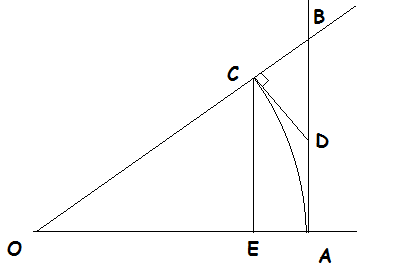
\includegraphics[width=0.40\textwidth]{LimSinx}
                    

                    Sea $x$ el angulo entre $BOA$

                    Primero supongamos que $OC = OA = 1$. Ahora, el camino mas corto de
                    $C$ a $OA$ es $CE$ que es $\Sin{x}$, pero otro camino es la longitud de
                    arco $CA$ que mide $x$ en radianes.

                    Entonces $\Sin{x} < x$.

                    Por otro lado, es obvio que la línea $BA$ es la $tan(x)$ y tenemos que
                    $\Tan{x} = BA = BD+DA > CD+DA > CA = x > \Sin{x}$.

                    Y ahí esta mi clave $\Sin{x} < x < \Tan{x}$.

                    Ahora si multiplicas todo por $\frac{1}{x}$ tenemos que 
                    $\frac{\Sin{x}}{x} < 1 < \frac{\Tan{x}}{x}$, por lo tanto 
                    $\frac{\Sin{x}}{x} < 1$.

                    Y como $1 < \frac{\tan{x}}{x} = \frac{\Sin{x}}{x} \frac{1}{\Cos{x}}$
                    entonces multiplicamos todo por $\Cos{x}$ y tenemos que $\Cos{x} < \Sin{x}{x}$

                    Entonces sabemos que $\Cos{x} < \Sin{x}{x} < 1$, ahora:
                    \begin{itemize}
                        \item $\lim_{x \to 0} \Cos{x} = 1$
                        \item $\lim_{x \to 0} 1 = 1$
                    \end{itemize}

                    Entonces $\Sin{x}{x}$ queda atrapada entre dos funciones que se aproximan a uno
                    cuando $x \to 0$, por lo tanto $\lim_{x \to 0} \dfrac{\Sin{x}}{x} = 1$
                                    
                \end{SmallIndentation}
                    
                


            % ==================================
            % =========   FORMAL     ===========
            % ==================================
            \clearpage
            \subsection{$\lim_{x \to 0} \dfrac{\Cos{x} - 1}{x}$}

                Esta es una de los dos límites más importantes en matemáticas, una de las claves para 
                resolver problemas y sobretodo para construir el concepto de derivadas.

                % ======== DEMOSTRACION ========
                \begin{SmallIndentation}[1em]
                    \textbf{Demostración}:
                    \begin{MultiLineEquation*}{3}
                        \lim_{x \to 0} \dfrac{\Cos{x} - 1}{x}
                            &= \lim_{x \to 0} \pfrac{\Cos{x} - 1}{x} (1)                            
                                && \Remember{Multiplicamos por inocente 1}                         \\
                            &= \lim_{x \to 0} \pfrac{\Cos{x} - 1}{x} \pfrac{\Cos{x}+1}{\Cos{x}+1}   
                                && \Remember{Transformamos el uno}                                  \\
                            &= \lim_{x \to 0} \pfrac{(\Cos{x} - 1)(\Cos{x}+1)}{x(\Cos{x}+1)}     
                                && \Remember{Metemos en la fracción}                                \\
                            &= \lim_{x \to 0} \pfrac{\Cos{x}^2 - 1}{x(\Cos{x}+1)}                   
                                && \Remember{Conjugado}                                             \\
                            &= \lim_{x \to 0} \pfrac{\Sin{x}^2}{x(\Cos{x}+1)}                       
                                && \Remember{$Pitagoras :\Cos{x}^2 -1 = \Sin{x}^2$}                 \\
                            &= \lim_{x \to 0} \pfrac{(\Sin{x}^2)x}{x^2(\Cos{x}+1)}                  
                                && \Remember{Creamos una x arriba y abajo}                          \\
                            &= \lim_{x \to 0} \pfrac{(\Sin{x}^2)}{x^2}\pfrac{x}{\Cos{x}+1}          
                                && \Remember{Separamos}                                             \\
                            &= \lim_{x \to 0} \pfrac{\Sin{x}}{x}^2 \pfrac{x}{\Cos{x}+1}           
                                && \Remember{Vemos que todo esta al cuadrado}                       \\
                            &= \lim_{x \to 0} (1)^2 \pfrac{x}{\Cos{x}+1}                            
                                && \Remember{Recuerda $\lim_{x\to 0} \frac{\Sin{x}}{x} = 0$}        \\
                            &= (1)^2 \pfrac{0}{\Cos{0}+1}                                           
                                && \Remember{Ya no hay indeterminaciones}                           \\
                            &= (1)^2 \pfrac{0}{1+1}                                                 
                                && \Remember{Algebra}                                               \\
                            &= (1)^2 (0)                                                            
                                && \Remember{Todo natural por cero es 0}                            \\
                            &= 0                                                                    
                                && \Remember{Tada! :D}                                              \\
                    \end{MultiLineEquation*}
                        
                
                \end{SmallIndentation}


                % ======== GEOMETRICA ========
                \clearpage
                \begin{SmallIndentation}[1em]
                    \textbf{Interpretación Geométrica}:


                    Este problema es muy importante porque con el podemos demostrar gran cantidad
                    de identidades, pero más que eso, también tiene una muy bonita interpretación
                    geométrica

                    \begin{figure}[h]
                        \centering
                        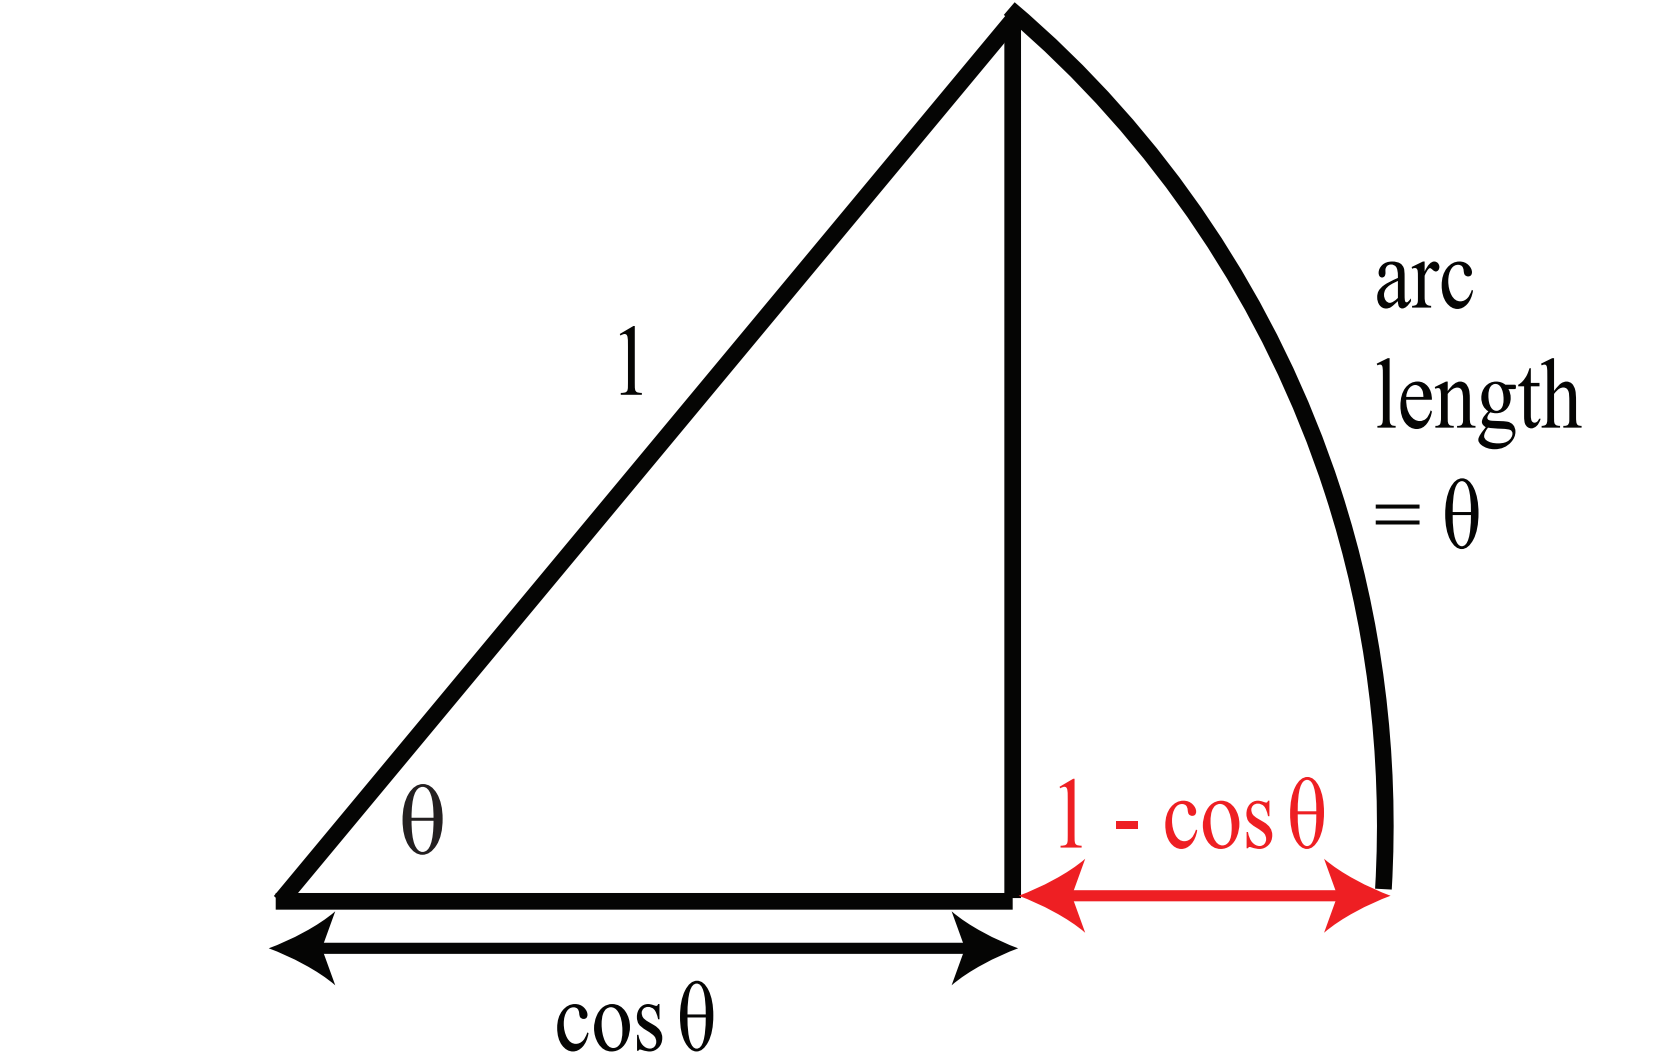
\includegraphics[width=0.45\textwidth]{LimCos-1}
                        \caption{Interpretación geométrica}
                    \end{figure}

                    Para enteder porque nuestro límite da eso, lo que tenemos que ver es
                    que podemos imaginar un circulo de radio uno, de tal manera, que si pusieramos
                    un triangulo rectangulo con un vertice en el origen y el otro tocando a la
                    circunferencia lo que pasaría sería que el otro lado mediría $\Cos{\theta}$

                    Y el espacio que le faltaría a ese vértice para tocar a la circunferencia es
                    $1-\Cos{\theta}$.

                    Lo que en realidad hacemos al momento de tomar el límite cuando $\theta \to 0$
                    es ver que pasa con esa distancia que le falta cuando la longitud de arco
                    de va haciendo más y más pequeña.

                    Y esta claro que mientras más pequeña sea la longitud de arco más pequeño será ese
                    espacio, de hecho podemos hacer que ese espacio se acerqué todo lo que queramos
                    a cero.  
                
                \end{SmallIndentation}
                    
                    




% ////////////////////////////////////////////////////////////////////////////////////////////////////////////////////
% //////////////////////////////////       CALCULO DIFERENCIAL       /////////////////////////////////////////////////
% ////////////////////////////////////////////////////////////////////////////////////////////////////////////////////
\part{Cálculo Diferencial}






% ////////////////////////////////////////////////////////////////////////////////////////////////////////////////////
% //////////////////////////////////       CALCULO INTEGRAL          /////////////////////////////////////////////////
% ////////////////////////////////////////////////////////////////////////////////////////////////////////////////////
\part{Cálculo Integral}

    % ======================================================================================
    % ========================  INTEGRACION IMPROPIA    ====================================
    % ======================================================================================
    \chapter{Integrales Impropias}
        \clearpage

        % =====================================================
        % ========         INTEGRACION IMPROPIA          ======
        % =====================================================
        \section{Integrales Impropias}

            Al definir la integral definida $\int_a^b f(x) dx$ estamos hablando
            de una función en la que:

            \begin{itemize}
                \item Esta definida en ese intervalo.
                \item No tiene una discontinuidad infinita
                \item Obviamente el intervalo es finito
            \end{itemize}

            Pero, que pasaría si no fuera así...

            Las integrales impropias explorar esta posibilidad así que veasmola:

        % ====================================================
        % ========== INTERVALOS INFINITOS ====================
        % ====================================================
        \clearpage
        \section{Tipo 1: Intervalos Infinitos}

            \subsubsection{Límite Superior}
            Si la $\int_a^t f(x) dx$ existe para todo número $t \geq a$, entonces
            lo siguiente es verdad, siempre que exista el límite (como un número finito).
            \begin{equation}
                \int_a^{\infty} f(x) dx = \lim_{t \to \infty} \int_a^t f(x) dx
            \end{equation}

            \subsubsection{Límite Inferior}
            Si la $\int_t^b f(x) dx$ existe para todo número $b \leq t$, entonces lo
            siguiente es verdad, siempre que exista el límite (como un número finito).
            \begin{equation}
                \int_{- \infty}^b f(x) dx = \lim_{t \to - \infty} \int_t^b f(x) dx
            \end{equation}

            \subsubsection{Convergencia}
            Las integrales impropias $\int_a^{\infty}f(x)dx$ y esta $\int_{-\infty}^bf(x)dx$
            se llaman \textbf{convegentes} si el límite existe y  \textbf{divergente} sino.

            \subsubsection{Ambos Límites}
            Si $\int_a^{\infty}f(x)dx$ y $\int_{-\infty}^bf(x)dx$ son convergentes, entonces
            se define esta asombrosa integral como:
            \begin{equation}
                \int_{-\infty}^{\infty} f(x) dx = \int_{-\infty}^{a} f(x) dx + \int_{a}^{\infty} f(x) dx   
            \end{equation}

            \subsubsection{Ejemplo}
            Podemos ver que con lo que sabemos ya podemos calcular la siguiente integral:

            \begin{equation*}
            \begin{split}
                \int_1^{\infty} \frac{1}{x^2} dx & = \lim_{t \to \infty} \int_1^t \frac{1}{x^2} dx \\
                & = \lim_{t \to \infty} \frac{-1}{x} \big\rvert_{1}^{t} \\
                & = \lim_{t \to \infty} \frac{-1}{t} - \frac{1}{-1} = \frac{-1}{t} + 1 = 1 + \frac{-1}{t} \\
                & = \lim_{t \to \infty} 1 + \frac{-1}{t} = 1 + 0 = 1
            \end{split}
            \end{equation*}

            \clearpage

        % ====================================================
        % ========== INTERVALOS INFINITOS ====================
        % ====================================================
        \clearpage
        \section{Tipo 2: Funciones Discontinuas}

            Si $f(x)$ es continua en $[a, b)$  pero discontinua en b, entonces
            (si el límite existe y es finito):
            \begin{equation}
                \int_a^b f(x) dx = \lim_{t \to b^-} \int_a^t f(x) dx
            \end{equation}

            Si $f(x)$ es continua en $(a, b]$  pero discontinua en a, entonces
            (si el límite existe y es finito):
            \begin{equation}
                \int_a^b f(x) dx = \lim_{t \to a^+} \int_t^b f(x) dx
            \end{equation}



            Si $\int_a^bf(x)dx$ es convergente, entonces se define esta asombrosa integral
            como (donde $c$ es $a<c<b$ ):
            \begin{equation}
                \int_a^b f(x) dx = \int_a^c f(x) dx + \int_c^b f(x) dx  
            \end{equation}


% ////////////////////////////////////////////////////////////////////////////////////////////////////////////////////
% //////////////////////////////////            CHEAT SHEET          /////////////////////////////////////////////////
% ////////////////////////////////////////////////////////////////////////////////////////////////////////////////////
\part{CheatSeet}

    % ==============================================================
    % ===============      PROPABILIDAD HARDCORE        ============
    % ==============================================================
    \clearpage
    \chapter{Reales}


        % ==============================================================
        % ===============            AXIOMAS                ============
        % ==============================================================
        \section{Axiomas}

        \begin{multicols}{2}
            \begin{enumerate}
                \item 
                    \textbf{Ley Aditiva Asociativa:}

                    $\forall a, b, c \in \Reals, \MiniSpace
                        (a + b) + c = a + (b + c)$

                \item 
                    \textbf{Ley Aditiva Conmutativa:}

                    $\forall a, b \in \Reals, \MiniSpace
                            a + b = b + a$

                \item 
                    \textbf{Elemento Indentidad Aditivo:}

                    $\exists 0 \in \Reals, \MiniSpace
                        \forall a \in \Reals, \MiniSpace 0 + a = a$

                \item 
                    \textbf{Existen Inversos Aditivos:}

                    $\forall a \in \Reals, \MiniSpace
                            \exists -a \in \Reals, \MiniSpace
                                a + (-a) = 0$

                \item 
                    \textbf{Ley Multiplicativa Conmutativa:}

                    $\forall a, b \in \Reals, \MiniSpace
                            ab = ba$

                \item 
                    \textbf{Ley Aditiva Asociativa:}

                    $\forall a, b, c \in \Reals, \MiniSpace
                        (ab)c = a(bc)$

                \item 
                    \textbf{Elemento Indentidad Multiplicativo:}

                    $\exists 1 \in \Reals, \MiniSpace
                        \forall a \in \Reals, \MiniSpace 1 \cdot a = a$

                \item 
                    \textbf{Existen Inversos Multiplicativos:}

                    $\forall a \in \Reals, \MiniSpace
                            \exists a^{-1} \in \Reals, \MiniSpace
                                a a^{-1} = 1$

                \item 
                    \textbf{Distributiva:}

                    $\forall a, b, c \in \Reals, \MiniSpace
                            a(b + c) = ab + ac \Also (a + b)c = ac + bc$

            \end{enumerate}

            \begin{itemize}

                \item Cancelación de la suma: 
                    Si $x, y, z \in \Reals$ tal que $x + z = y + z$, entonces $x = y$

                \item El neutro aditivo es único

                \item El inverso aditivo de $a$ es único

                \item $\forall a \in \Reals, \MiniSpace a \cdot 0 = 0$

                \item $\forall a \in \Reals,  -(-a) = a$

                \item $\forall a \in \Reals,  -a = (-1)a$

                \item $\forall a, b \in \Reals, a(-b) = -(ab) = (-a)b$

                \item $-0 = 0$

                \item Sea $a, b \in \Reals$ entonces $ab = 0$ si y solo si $a=0$ ó $b=0$

                \item Sea $ab = ac$ y $a \neq 0$ entonces $b = c$

                \item Sea $(ab)^{-1} = a^{-1}b^{-1}$

            \end{itemize}

        \end{multicols}

        
        % ==============================================================
        % ===============         RESTA Y DIVISION          ============
        % ==============================================================
        \clearpage
        \section{Resta y División}

            \begin{itemize}
                \item 
                    Definimos a $a - b := a + (-b)$
                \item
                    Definimos a $\frac{a}{b} := ab^{-1}$ si es que $b \neq 0$
                    porque $0^{-1}$ no existe
            \end{itemize}

            \begin{itemize}
                \item $\pfrac{a}{b} \pfrac{c}{d} = \dfrac{ac}{bd}$ si $b \neq 0$ y $d \neq 0$
                    
                \item $\forall a, b, c, d \in \Reals$ tal que $b \neq 0$ y $d \neq 0$ entonces
                        $\dfrac{a}{b} + \dfrac{c}{d} = \dfrac{ad+bc}{bd}$        

                \item $\forall a, b \in \Reals$ $a^2-b^2 = (a+b)(a-b)$

                \item $\forall a, b \in \Reals$ Si $a^2 = b^2$ entonces $a=b$ o $a=-b$

            \end{itemize}


        % ==============================================================
        % ===============        TRICONOMIA Y ORDEN         ============
        % ==============================================================
        \clearpage
        \section{Tricotomía y Orden}

            Vamos a igual suponer como axioma la siguiente afirmación:

            Sea $P$ un conjunto elemental, compuesto por todos los reales positivos, entonces 
            para todo $a, b \in \Reals$ pasa una y solo una de las siguientes cosas:

            \begin{itemize}
                \item $a \in P$
                \item $-a \in P$
                \item $a = 0$
            \end{itemize}

            Ahora es importante ver como se comportan $P$, en especial estos 2 axiomas:
            \begin{itemize}
                \item Es cerrado bajo la suma, es decir $\forall a, b \in P \MiniSpace a + b \in P$
                \item Es cerrado bajo la multiplicación, es decir $\forall a, b \in P \MiniSpace ab \in P$
            \end{itemize}


            \begin{itemize}
                \item Transitividad. Si $a < b$ y $b < c$ entonces $a < c$
                \item Si $a < b$ y $c \in \Reals$ entonces $a+c < b+c$
                \item Si $a < b$ y $c < d$ entonces $a+c < b+d$
                \item Si $a < b$ y $c > 0$ entonces $ac < bc$
                \item Si $a < b$ y $c < 0$ entonces $ac > bc$
                \item Si $a \neq 0$ entonces $a^2 > 0$
                \item Si $0 \leq a < b$ y $0 \leq c < d$ entonces $ac < bd$
                \item Si $a < b$ entonces $-a > -b$
            \end{itemize}

        % =====================================================
        % ==========     POTENCIAS Y RAICES          ==========
        % =====================================================
        \clearpage
        \section{Potencias y Raíces}


            Si $x \in \Reals$ entonces:
            \begin{MultiLineEquation*}{3}
                |x| = 
                \begin{cases} 
                    x & \text{si $x \geq 0$}    \\
                    -x & \text{si $x < 0$}
                \end{cases}
            \end{MultiLineEquation*}
                

            \begin{itemize}
                \item Sea $a \in \Reals$ y sea $b = a \cdot a$ entonces $\sqrt{b} := |a|$
                \item Sea $a, b \in \Reals$ con $b \geq 0$y entonces $\sqrt{a} := b$ si y solo si $a=b^2$
            \end{itemize}

            \begin{itemize}

                    \item $a < \sqrt{ab} < \dfrac{a+b}{2} < b$

                    \item $a = (\sqrt{a})^2$

                    \item Si $b \geq 0$ entonces $a^2 > b$ si y solo si $a>\sqrt{b}$ o $a<-\sqrt{b}$

                    \item $|a| \geq 0 \Space \forall a \in \Reals$

                    \item $|a| = 0 \lEqual a = 0$
                    
                    \item $|a| = |-a|$
                    
                    \item $a^2 = |a|^2 = |a^2|$
                    
                    \item $|a+b| \geq |a\| + |b|$
                    
                    \item $|a-b| \geq |a\| - |b|$
                    
                    \item $|a||b| = |ab|$

                    \item $|a| = |b| \lEqual a = b$ o $a = -b$

                    \item $|a| = b \lEqual a = b$ o $a = -b$

                    \item $|a| < b \lEqual -b < a < b$
                    \item $|a| > b \lEqual a < -c $ o $a > c$

            \end{itemize}

        



\end{document}